\chapter{Lecture 18}
In this lecture, we discuss model complexity. Model complexity can fall into many categories including, but not limited to, the following items.
\begin{itemize}
    \item Analysis 
    \item Can the model be approximated well with a simpler model?
    \item How costly is the model to compute?
    \begin{itemize}
        \item Computational complexity for problem class (e.g., P or NP?)
        \item Computer time cost 
        \item Basic operation count (number of floating point operations)
        \item Memory requirements (e.g., solving linear system iteratively requires less memory than LU factorization)
        \item Parallelizability
    \end{itemize}
\end{itemize}
Note that regarding computing cost, we often consider worst-case, best-case, and average-case scenarios. For example, for optimizing a function $f$, simplex methods have a very large worst-case cost but have reasonable average-case cost.
\section{Complexity Classes} \label{sec:18:complexity}
We discuss a two complexity classes pertinent to computational science: $P$ and $NP$. Note that the following discussion is not fully rigorous as we do not present the formalism of Turing machines. To the interested reader, we refer to Michael Sipser's introductory text \cite{sipser1996introduction}. 
\begin{definition}{(Polynomial-Time Algorithm)} \label{def:18:poly}
We say that an algorithm $\mathcal{A}$ is a polynomial-time algorithm for problem $\mathcal{P}$ if and only if there exists $C \geq 0$, $\alpha \geq 0$, and $N_0 \in \mathbb{N}$ such that for any all inputs $\mathcal{I}$ of size $N \geq N_0$, simulating $\mathcal{A}$ with input $\mathcal{I}$ computes $\mathcal{P}(\mathcal{I})$ with computational time cost no more than $C N^{\alpha}$. 
\end{definition}
As the name suggests, a polynomial-time algorithm is one which has cost no worse than some polynomial, even if the polynomial grows quickly. Of course, for any problem, there exist algorithms that are worse than polynomial-time algorithms (we can sit idle for as long as we like and only then compute the solution), but this is not generally interesting. What is interesting is the existence of a polynomial-time algorithm for a given problem. This class is precisely the class $P$.
\begin{definition}{(Complexity Class $P$)} 
A problem $\mathcal{P}$ lies in the complexity class $P$ if and only there exists a polynomial-time algorithm for $\mathcal{P}$. 
\end{definition}
In some sense, $P$ can be thought of as a set of problems for which solutions can be found \q{quickly}. In this context, \q{quickly} means precisely \q{has a polynomial-time algorithm.} We are now ready to define $NP$.
\begin{definition}{(Complexity Class $NP$)}
A problem $\mathcal{P}$ lies in the complexity class $NP$ if and only if there exists a polynomial-time algorithm $\mathcal{A}$ that solves the following auxiliary problem $Q$: given any tuple $(\mathcal{I}, \mathcal{O})$, $\mathcal{P}(\mathcal{I}) = \mathcal{O}$? 
\end{definition}
$NP$ can thus be thought of as any problem where checking whether a solution is correct or not can be verified \q{quickly.} However, finding the solution the problem given any input is not necessarily a \q{quick} operation. Note that $P \subseteq NP$. But $NP \subseteq P$? The answer to this is still an open question and is, in fact, a Clay Millennial Prize problem worth one million dollars! 

A familiar example of an $NP$ problem is solving an $n \times n$ Sudoko puzzle. As the size of the puzzle grows, the number of possibilities that we must check grows exponentially. However, verifying if a particular guess is correct can be done in $O(n^2) = O(N)$ time (linear because our input size is $N=n^2$). We simply check every row and every column and if we ever see a contradiction, we output false. If we never run into one, we output true. This suggests that if we were to have some special insight to \q{zoom in} on the correct answer at the start, we would have a polynomial-time algorithm that solves Sudoko and thus that problem lies in $P$. However, nobody has ever constructed such an algorithm and many experts in this field suspect that $P \neq NP$. If $P \neq NP$, this suggests that there is some inherent complexity to the \q{search process}, and there is no \q{quick} way to \q{zoom in} on the correct solution, even if that correct solution can be verified \q{quickly}.

\section{Complexity Back Down on Earth}
The discussion above lies at the heart of theoretical computer science, but we now return to complexity theory as it pertains to applied mathematics and computational scientists. 
While $O(N^{2})$ and $O(N)$ algorithms are essentially the same to theoretical computer scientist trying to solve the $P=NP$ problem, the former is, in certain cases, unacceptably expensive and the latter what computational scientists strive for. 
This motivates the question \q{given a model, is there inherent complexity that prevents it from ever being used in practice?} Typically, we are interested in time complexity and memory complexity. Time complexity is usually expressed in terms of floating point operations (FLOPs). Memory complexity is usually expressed in terms of bytes, megabytes, gigabytes, or terabytes, depending on the scale.

\subsection{Sparse Matrix Inversion}
Consider the problem of solving 
\begin{equation} \label{eqn:18:sparse}
\bs{A} \bs{x} = \bs{b}
\end{equation}
where $\bs{A} \in \R^{N \times N}$ is sparse, i.e., has $O(N)$ nonzero entries. Computing a na\"{i}ve LU decomposition immediately loses the sparse structure with $O(\frac{2}{3}N^3)$ FLOPs for the construction and backsubstitution and memory cost of $O(2N^2)$. For large $N$, the cubic complexity will often be prohibitively costly in addition to the quadratic memory cost. This setting is more natural for an iterative solver such as GMRES. All that needs to be computed is the action of the matrix $\bs{A}$ on a given vector $\bs{x}$. Since $\bs{A}$ is sparse, this is an $O(N)$ operation. Furthermore, the storage requirement is just $O(N)$ also.\footnote{Note that in certain contexts, this may even be improved to $O(1)$! For example, consider the Laplacian matrix which is tridiagonal matrix with repeated entries $-1$,$2$, and $-1$. Its action thus requires \bt{no} memory since we can even hardcode the numbers $-1$ and $2$ directly into our program!}
If the iterative solver converges in a few iterations, we have a $O(N)$ algorithm for a problem whose na\"{i}ve approach is $O(N^3)$! Note further that when $A$ is symmetric, positive-definite, and real, then our iterative solver can be chosen to be the conjugate gradient method which is guaranteed to converge in $N$ steps.\footnote{In general, as long as $\bs{A}$ is invertible, then we can recast to the normal equations and apply conjugate gradient to the system
\begin{equation*}
    \bs{A}^{*} \bs{A} \bs{x} = \bs{A}^{*}\bs{b}
\end{equation*}
} 
This leads to an overall complexity of $O(N^2)$ in the worst case, which is still a drastic reduction in complexity!

\subsection{Sparse Matrix Inversion on a GPU}
Let us consider the memory requirement associated with sparse matrix inversion. Say we have an Nvidia A100 80GB chip (state-of-the-art as of when this was written in May 2022). 80GB will store $20$ billion single-precision floating point numbers. Direct $LU$ decomposition will require $2N^2$ entries. Therefore, the maximal value of $N$ that we could store $N = \sqrt{\frac{20 \times 10^9}{2}} = 100,000$.\footnote{Note that this is an optimistic estimate given that, in practice, we need other parts of memory for other tasks on the GPU such as performing back substitution once the factors $L$ and $U$ have been constructed.} However, if our matrix is sparse, say with $3N$ nonzero entries, then we can consider problems of size up to $N = \frac{20 \times 10^{9}}{3} \approx 6.6$ billion!\footnote{Again, with the same caveat as the previous footnote.} 

\section{Structural Complexity}
In addition to time and memory complexity, we sometimes refer to model complexity. For example, linear problems tend to be less complex than nonlinear ones. ODEs tend to be less complex than PDEs and SDEs. 

\section{Information Theory}
Information theory is the study of quantifying the complexity inherent to a model or problem. In short, it can be viewed as the minimal number of bits to represent all states of a model or problem. For example, the bit string 
\begin{align} \label{eqn:18:simpleprogram}
    0101010101010\underbrace{...}_{\txt{repeats}}
\end{align}
can be encoded in just three numbers $0$, $1$, and $2$ (the stride length of repeating). On the other hand, the bit string 
\begin{align} \label{eqn:18:complexprogram}
    001101010101010001011111101010011110\underbrace{...}_{\txt{repeats}}
\end{align}
can be encoded with $38$ numbers, $37$ for the pattern displayed and one number to store the stride length of $37$. 
These examples have at most a complexity of $3$ numbers and $38$ numbers, respectively.
A fundamental result of information theory that is of importance to applied mathematics is the Nyquist-Shannon Theorem and its associated interpolation formula.
\cbeqn{Nyquist-Shannon sampling theorem}{
    \txt{If } f \txt{ is bandlimited by } B > 0 \txt{, i.e., } supp(\mathcal{F}(f)) \subseteq [-B,B], \txt{ then } \label{eqn:18:nyquistsampling} \\
    f \txt{ is }  \txt{recovered by uniform samples with step size } \Delta t = \frac{1}{2B} \nonumber
}
\cbeqn{Shannon-Whittaker interpolation formula}{
    \txt{If } f,B,\Delta t \txt{ are as in } \pref{eqn:18:nyquistsampling}, \txt{then } \label{eqn:18:shannoninterp} \\
        f(t) = \sum_{n=-\infty}^{\infty} f(n \Delta t) sinc\left(\frac{f - n \Delta t}{\Delta t}\right) \nonumber
}
This theorem has impact on computational complexity regarding the number of grid points needed in FEM, FDM, and FVM. If sampling is done more coarsely than outlined in Equation \pref{eqn:18:shannoninterp}, then any algorithm will output garbage.\footnote{Note that this does not guarantee good results if sampled more finely! It is only the bare minimum for recovery!} The Nyquist-Shannon sampling theorem shines light on the inherent complexity of some multiscale problems. For high frequency modes, the sampling rate increases according to the Nyquist frequency.

\subsection{Propagation of Light}
We consider the problem of light propagation as applied to computer graphics. A hierarchy of models for this process are outlined below.
\begin{enumerate}
    \item Ray tracing (Geometric Optics)
        \begin{enumerate}
            \item Follow individual light rays
            \item High-frequency approximation of wave equation
        \end{enumerate}
    \item Wave equation
    \item Quantum mechanics
\end{enumerate}
Ray tracing is the lowest-order approximation to the physics of light propagation. We simply take a light source and discretize it into many rays. Then we follow those rays within their environment to create a picture of the lighting of the scene, finding which rays end up entering the eye of our an observer placed at a desired point of view. A schematic of this process is show in Figure \ref{fig:18:raytracing}. Its low complexity makes it an industry-standard for lighting scenes for computer graphics. Although directly solving a wave equation would, in theory, be a more accurate model, we can show with a back-of-the-envelope calculation that this is infeasible. Light has a wavelength of roughly $500$ nanometers if we take the middle of the visible spectrum. For a cubic room of one cubic meter, to sample down to the Nyquist wavenumber,\footnote{This is typically referred to as the Nyquist frequency because we typically think in terms of a time series, in which case the Fourier domain is a frequency domain. However, here we are think of a spatial signal, so the Fourier domain is the wavenumber domain} we thus need to take 
\begin{align*}
O\left[\left(\frac{1}{2 * 5 * 10^{-7}}\right)^{3}\right]=O(10^{18}) \txt{ samples!} 
\end{align*}
\askbjorn{Double check calculation...it looks like \bjorn dropped the $500$ term which changes the calculation significantly, albeit is quite expensive still}
In the extremely optimistic case where we have a linear solver for the wave equation, we still would need an exascale computer to light the scene. Even worse, if we can only get a quadratic solver, then this problem is completely infeasible, requiring $O(10^{36})$ FLOPs. Finally, we are often interested in moving the point of view around the scene, so this task would certainly be infeasible for a task such as real-time ray tracing.\footnote{Typically for movies, developers spend a long time rendering very detailed scences and then stitch them together as one continuous movie. This is partially why animated movies take so long to make. However, real-time ray tracing aims at being able to re-render a scene as quickly as a user might move the point of view of the scene. When I learned about real-time ray tracing for the first time in 2015, it still had not been fully realized but was (and still is) an active area of research. However, computers have gotten fast enough to make this feasible as of today (2022).} \askbjorn{Ray tracing certainly does not capture this information either though; it sort \q{sidesteps} the issue of Nyquist frequency by using a high-frequency approximation. Should we comment on this?} A natural question is \q{how well does the ray-tracing approximation work in practice?} Nvidia recently (as of 2019) released another installation of \textit{Project Sol} whose goal was to exhibit real-time ray tracing for a cinematic scene. It was a fantastic success, and the video can be seen at this \href{https://www.youtube.com/watch?v=pNmhJx8yPLk}{link}. This video is very realistic and should be convincing that the ray tracing approximation is sufficiently accurate for computer graphics applications.
\begin{figure}
    \centering
    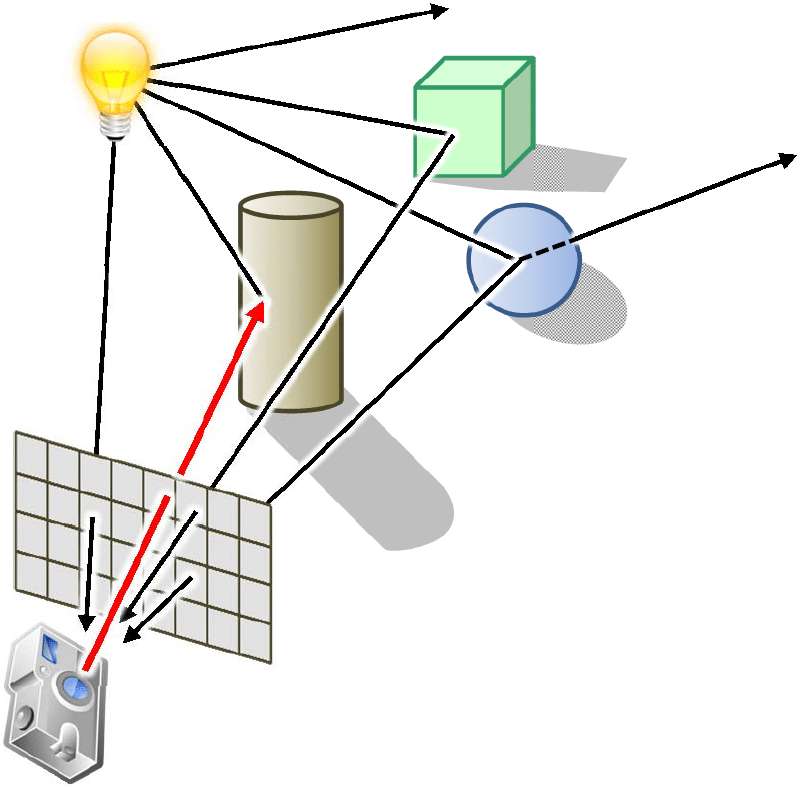
\includegraphics[width=\textwidth]{images/RayTracing.png}
    \caption{A schematic of ray tracing taken from computer graphics paper \cite{retzlaff2017physically}}
    \label{fig:18:raytracing}
\end{figure}
\section{Kolmogorov complexity and Kolmogorov $n$-width}
Recall that a reduced-order model (ROM) is an attempt to create a cheaper model that accurately approximates a more complex model. The inherent complexity of a model can be summarized by its \bt{Kolmogorov complexity}. In short, the Kolmogorov complexity is \q{the length of the shortest computer program that solves the problem.} It is the formalization of the introductory discussion of this section how cheaply we can store the information contained in the bit strings in Equations \eqref{eqn:18:simpleprogram} and \eqref{eqn:18:complexprogram}. 

The \bt{Kolmogorov $n$-width} of an object is a measure of how close an object is to its model approximation in lower dimensional space \askbjorn{Double check wording here}. Let $X$ be a normed linear space.
\begin{definition}{(Distance between point and subspace)}
Then we define the distance from a point $x \in X$ to an $n$-dimensional subspace $X_n \leq X$ as
\begin{align*}
    dist(x,X_n) := \inf_{y_n \in X_n} \|x - y_n\|_{X}.
\end{align*}
\end{definition}
This concept can be generalized to a subset $A \subseteq X$. It is defined as the largest distance from a point $x \in A$ to the subspace $X_n$. 
\begin{definition}{(Distance between subset and subspace)}
The distance between a subset $A \subseteq X$ and the $n$-dimensional subspace $X_n \leq X$ is defined as
\begin{align*}
    dist(A, X_n) := \sup_{x \in A} dist(x,X_n) = \sup_{x \in A} \left( \inf_{y_n \in X_n} \|x-y_n\|_{X} \right)
\end{align*}
\end{definition}
Finally, we are ready to define Kolmogorov $n$-width.
\begin{definition}{(Kolmogorov $n$-width)}
The Kolmogorov $n$-width of a set $A \subseteq X$ with respect to the normed space $X$\footnote{Note that the space $X$ and its associated norm $\|\cdot\|_{X}$ affects this computation.} is defined as
\begin{align*}
    d_{n}(A, X) &:= \inf_{\underset{dim(X_n)=n}{X_n \leq X}} dist(A,X_n) \\
        &= \inf_{\underset{dim(X_n)=n}{X_n \leq X}} \left[ \sup_{x \in A} \left( \inf_{y_n \in X_n} \|x - y_n\|_{X} \right)\right]
\end{align*}
\end{definition}
\askbjorn{Compare POD}
